\documentclass[tikz,border=10pt]{standalone}
\usetikzlibrary{angles,quotes}

\begin{document}
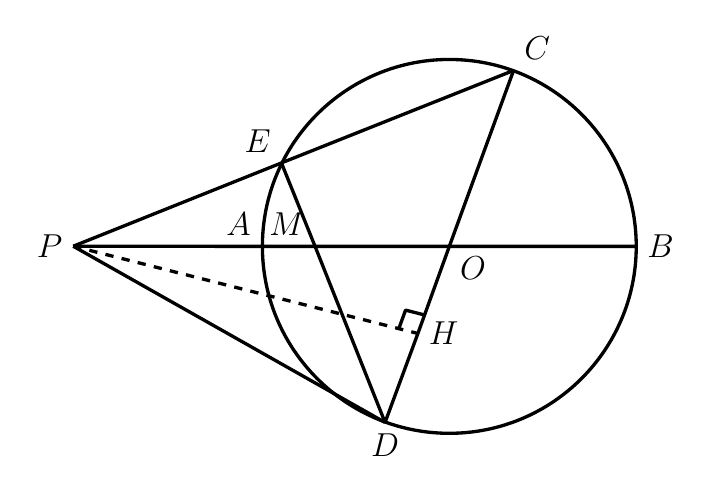
\begin{tikzpicture}[line width=1.2pt, line join=round, font=\fontsize{12}{14.4}\selectfont]
\coordinate (A) at (-1.206,0.008);
\coordinate (B) at (3.553,0.008);
\coordinate (C) at (1.993,2.242);
\coordinate (D) at (0.361,-2.228);
\coordinate (E) at (-0.955,1.068);
\coordinate (H) at (0.778,-1.098);
\coordinate (M) at (-0.528,0.008);
\coordinate (O) at (1.177,0.008);
\coordinate (P) at (-3.599,0.010);











  
  \draw (P) -- (A) -- (M) -- (O) -- (B);

  
  \draw (P) -- (E) -- (C);

  
  \draw (C) -- (O) -- (H) -- (D);

  
  \draw (P) -- (D);
  \draw (E) -- (M) -- (D);

  
  \draw (O) circle (2.374);

  
  \draw[dashed] (P) -- (H);
  \draw pic[draw, angle radius=0.250cm] {right angle=P--H--C};

  
  \node[left] at (P) {$P$};
  \node[above left] at (A) {$A$};
  \node[above left] at (M) {$M$};
  \node[below right] at (O) {$O$};
  \node[right] at (B) {$B$};
  \node[above left] at (E) {$E$};
  \node[above right] at (C) {$C$};
  \node[below] at (D) {$D$};
  \node[right] at (H) {$H$};
\end{tikzpicture}
\end{document}